\documentclass[../tech_report_1.tex]{subfiles}
\graphicspath{{img/}{../img/}}
\begin{document}

Shape analysis is the fundamental computer vision problem of helping machines understand shape. Here, we focus primarily on the subproblem of shape retrieval: given a \textit{query shape}, how can we best retrieve the most similar shapes (\textit{search results}) from an already-known catalog of shapes? Shape retrieval is as similarly fundamental to the problem of shape analysis as search engines to was to the Internet.

The standard general framework for shape retrieval is to consume some shape representation (e.g. 2D points, 3D point-clouds, or 3D meshes), extract a feature representation that captures the essence of the shape, and use retrieval mechanics to output a list of shapes based on similarity.

\section{Motivations}

There has been several developments which make shape analysis both exciting and crucial in recent years. First, the number of available models (2D and 3D shapes) available over the Internet, partly due to ever-decreasing costs of creating such models and partly due to the concerted efforts of researchers to construct domain-specific databases. Second, our understanding of the principles behind computer vision have advanced greatly, due to both the necessity of making sense of enormous amount of data being generated every day \cite{manyika2011big}, and meteoric advances in our ability to solve them \cite{krizhevsky2012imagenet}.

It is interesting to note that, fundamentally, our understanding of images and objects comes directly from our ability to understand their shape. To see this most intuitively, consider the two versions of the same picture in figures \ref{figure:still_life_original} and \ref{figure:still_life_outline} which we immediately recognize as containing the same semantic meaning, despite the stripping away of most attributes in \ref{figure:still_life_outline}. We could change the speed, scale, amount of distortion, and almost any other characteristic parameter and still retain the same meaning.

\begin{figure}[H]
	\centering
	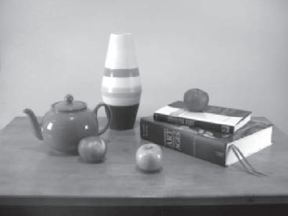
\includegraphics{still_life_full}
	\caption{Original photograph of still life\label{figure:still_life_original}}
\end{figure}

\begin{figure}[H]
	\centering
	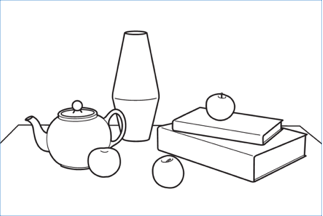
\includegraphics{still_life_outline}
	\caption{Same scene with purely shape information\label{figure:still_life_outline}}
\end{figure}


\section{Applications}

Shape retrieval has a plethora of potential applications, which stems from how fundamental shape analysis is to the problem of computer vision. Solving shape retrieval has as far ranging effects as helping robots quickly make sense of their environment, helping build billion-dollar 3D animation franchises, and becoming an enabler of information retrieval for commerce and virtual/augmented reality on the scale that search engines did for text-based websites. Ultimately, fully understanding the implications of solving this problem may be impossible because the problem is so basic.

\end{document}
